\section{Subtractor}
Før brugen af subtractoren har vi et signal, der er forstærket op til 4V. Med dette signal bruges indgangen -4V til 4V på AD-Converteren. Ved kun at bruge 0-4V gør det, at vi kommer til at miste én af NI-DAQ 6009's 14 bit. For at forhindre dette bruges en subtractor til at trække signalet ned, så det i stedet for at gå fra 0-4V går fra -2-2V. Dette giver os muligheden for at bruge indgangen -2,5-2,5V på AD-Converteren. Vi kan med dette forhindre, at vi kommer til at miste en bit. Til subtractoren benytter vi operationsforstærkeren OP27GH.

\subsection{Beregninger}
\vspace{0.2cm}
På vores kredsløb for subtractoren kan vi først slukke for v2, så vi får et udtryk for vO1.
\[ V_{O1}=-\frac{R2}{R1}\cdot V_{1} \]

Nu slukker vi for v1 og får dermed et udtryk for vO2.
\[ V_{O1}=[\frac{R4}{R3+R4}]\cdot [\frac{R1+R2}{R1}] \cdot V_{2} \]

Ved brug af superposition tilføjer vi vores ønskede outputs på vores to kilder
\[ V_{O}=V_{O1}+V_{O2} \]

Vi kan nu indsætte værdierne for $V_{O1}$ og $V_{O2}$. 
\[ V_{O}=-\frac{R2}{R1}\cdot V_{1}+[\frac{R4}{R3+R4}]\cdot [\frac{R1+R2}{R1}] \cdot V_{2} \]

De fire modstande bestemmes med samme værdier. Værdien vælges til 10k$\Omega$
\[ R1=1000k\Omega \]
\[ R2=1000k\Omega \]
\[ R3=1000k\Omega \]
\[ R4=1000k\Omega \]

Dette gør, at de fire modstande divideret med hinanden giver 1.
\[ \frac{R3}{R1}=\frac{R4}{R2} = 1 \]

Dette kan vi benytte i funktionen for $V_{O}.$
\[ V_{O}=V_{2}-V_{1} \]

$V_{2}$ er input i subtractoren og $V_{1}$ er spændingen vi ønsker at nedjustere vores signal med.
\[ V_{O}=4V-2V=2V \]

\clearpage

\subsection{Test af subtractor}
Til at teste subtractoren på fumlebræt bruges waveforms til at generere to signaler - et DC signal med 2V, der her fungerer som subtractorens $V_{1}$ samt et sinus signal. Signaler med henholdsvis 2V amplitude og offset 2V til at vise 0-4V og et med amplitude 2V og offset 3V til at vise 1-5V. På figurerne neden for ses det, at subtractoren trækker begge signaler ned med 2V, så det første signal viser -2-2V og det andet signal viser -1-3V.

\begin{figure}[h!]
	\centering
	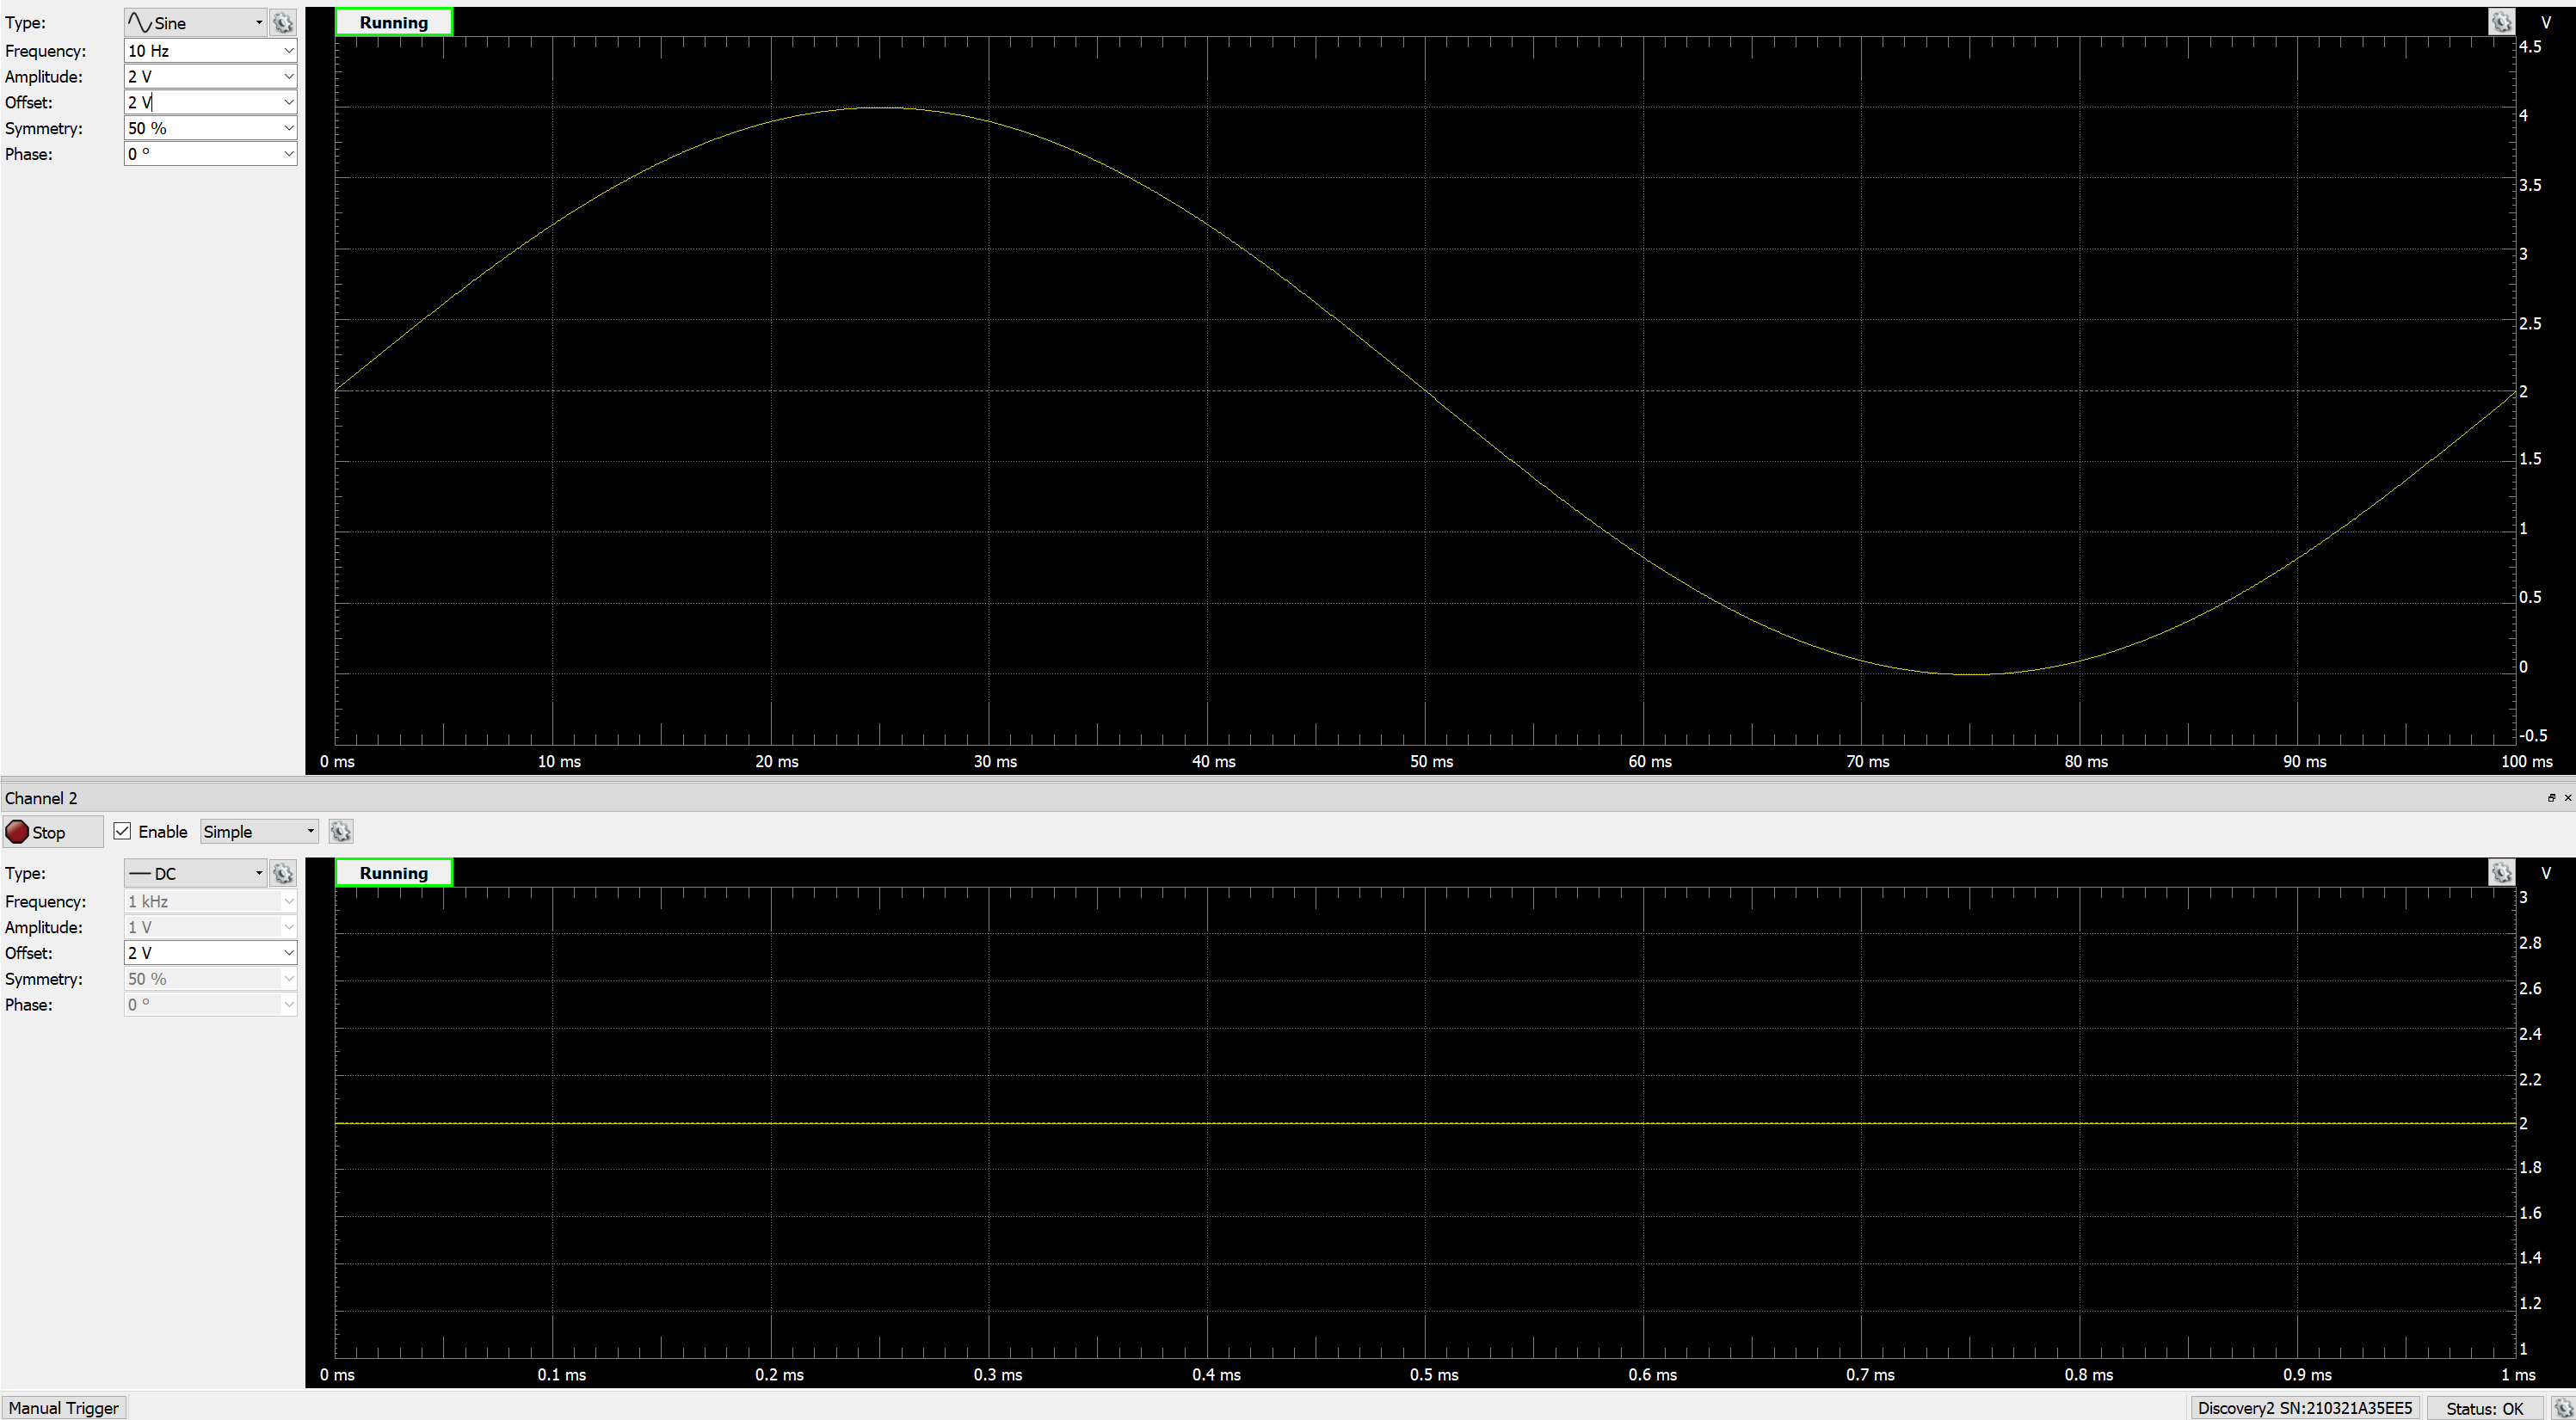
\includegraphics[width=1\linewidth]{Hardwaredesign/Subtractor1}
	\caption{Test af subtractor - offset 2V}
	\label{fig:Subtractor1}
\end{figure}

\begin{figure}[h!]
	\centering
	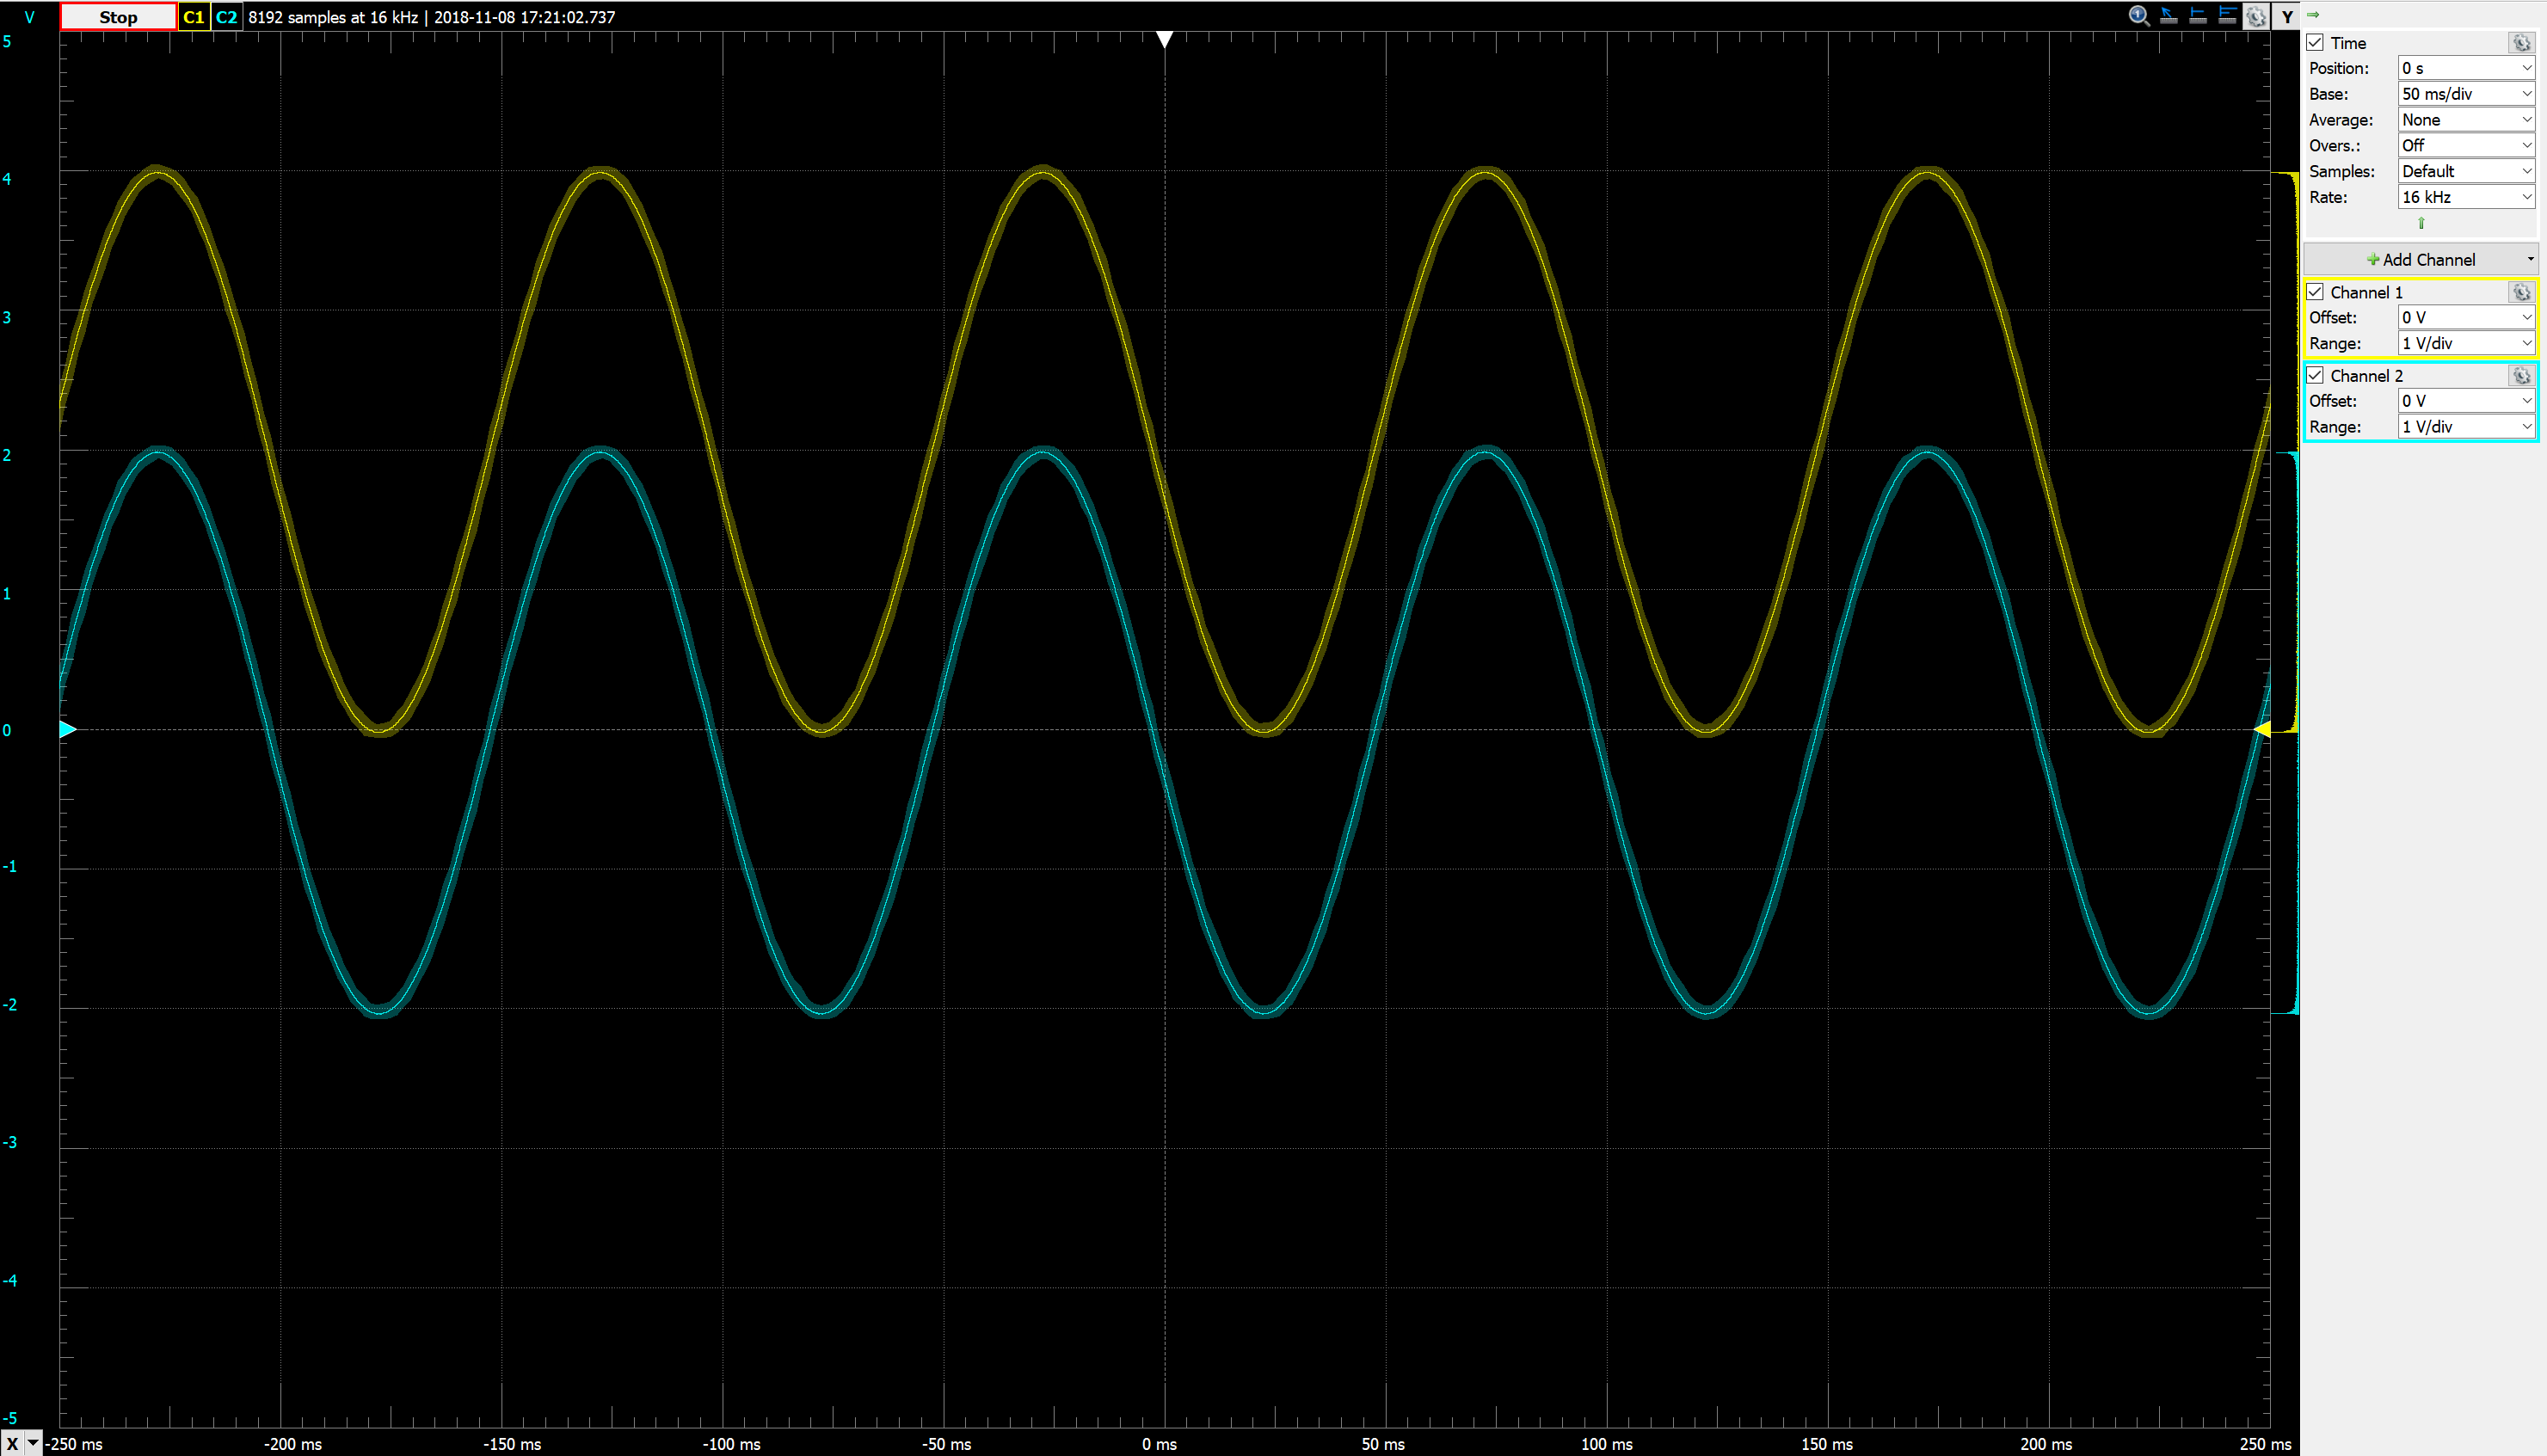
\includegraphics[width=1\linewidth]{Hardwaredesign/Subtractor2}
	\caption{Test af subtractor - offset 2V}
	\label{fig:Subtractor2}
\end{figure}

\clearpage
\begin{figure}[h!]
	\centering
	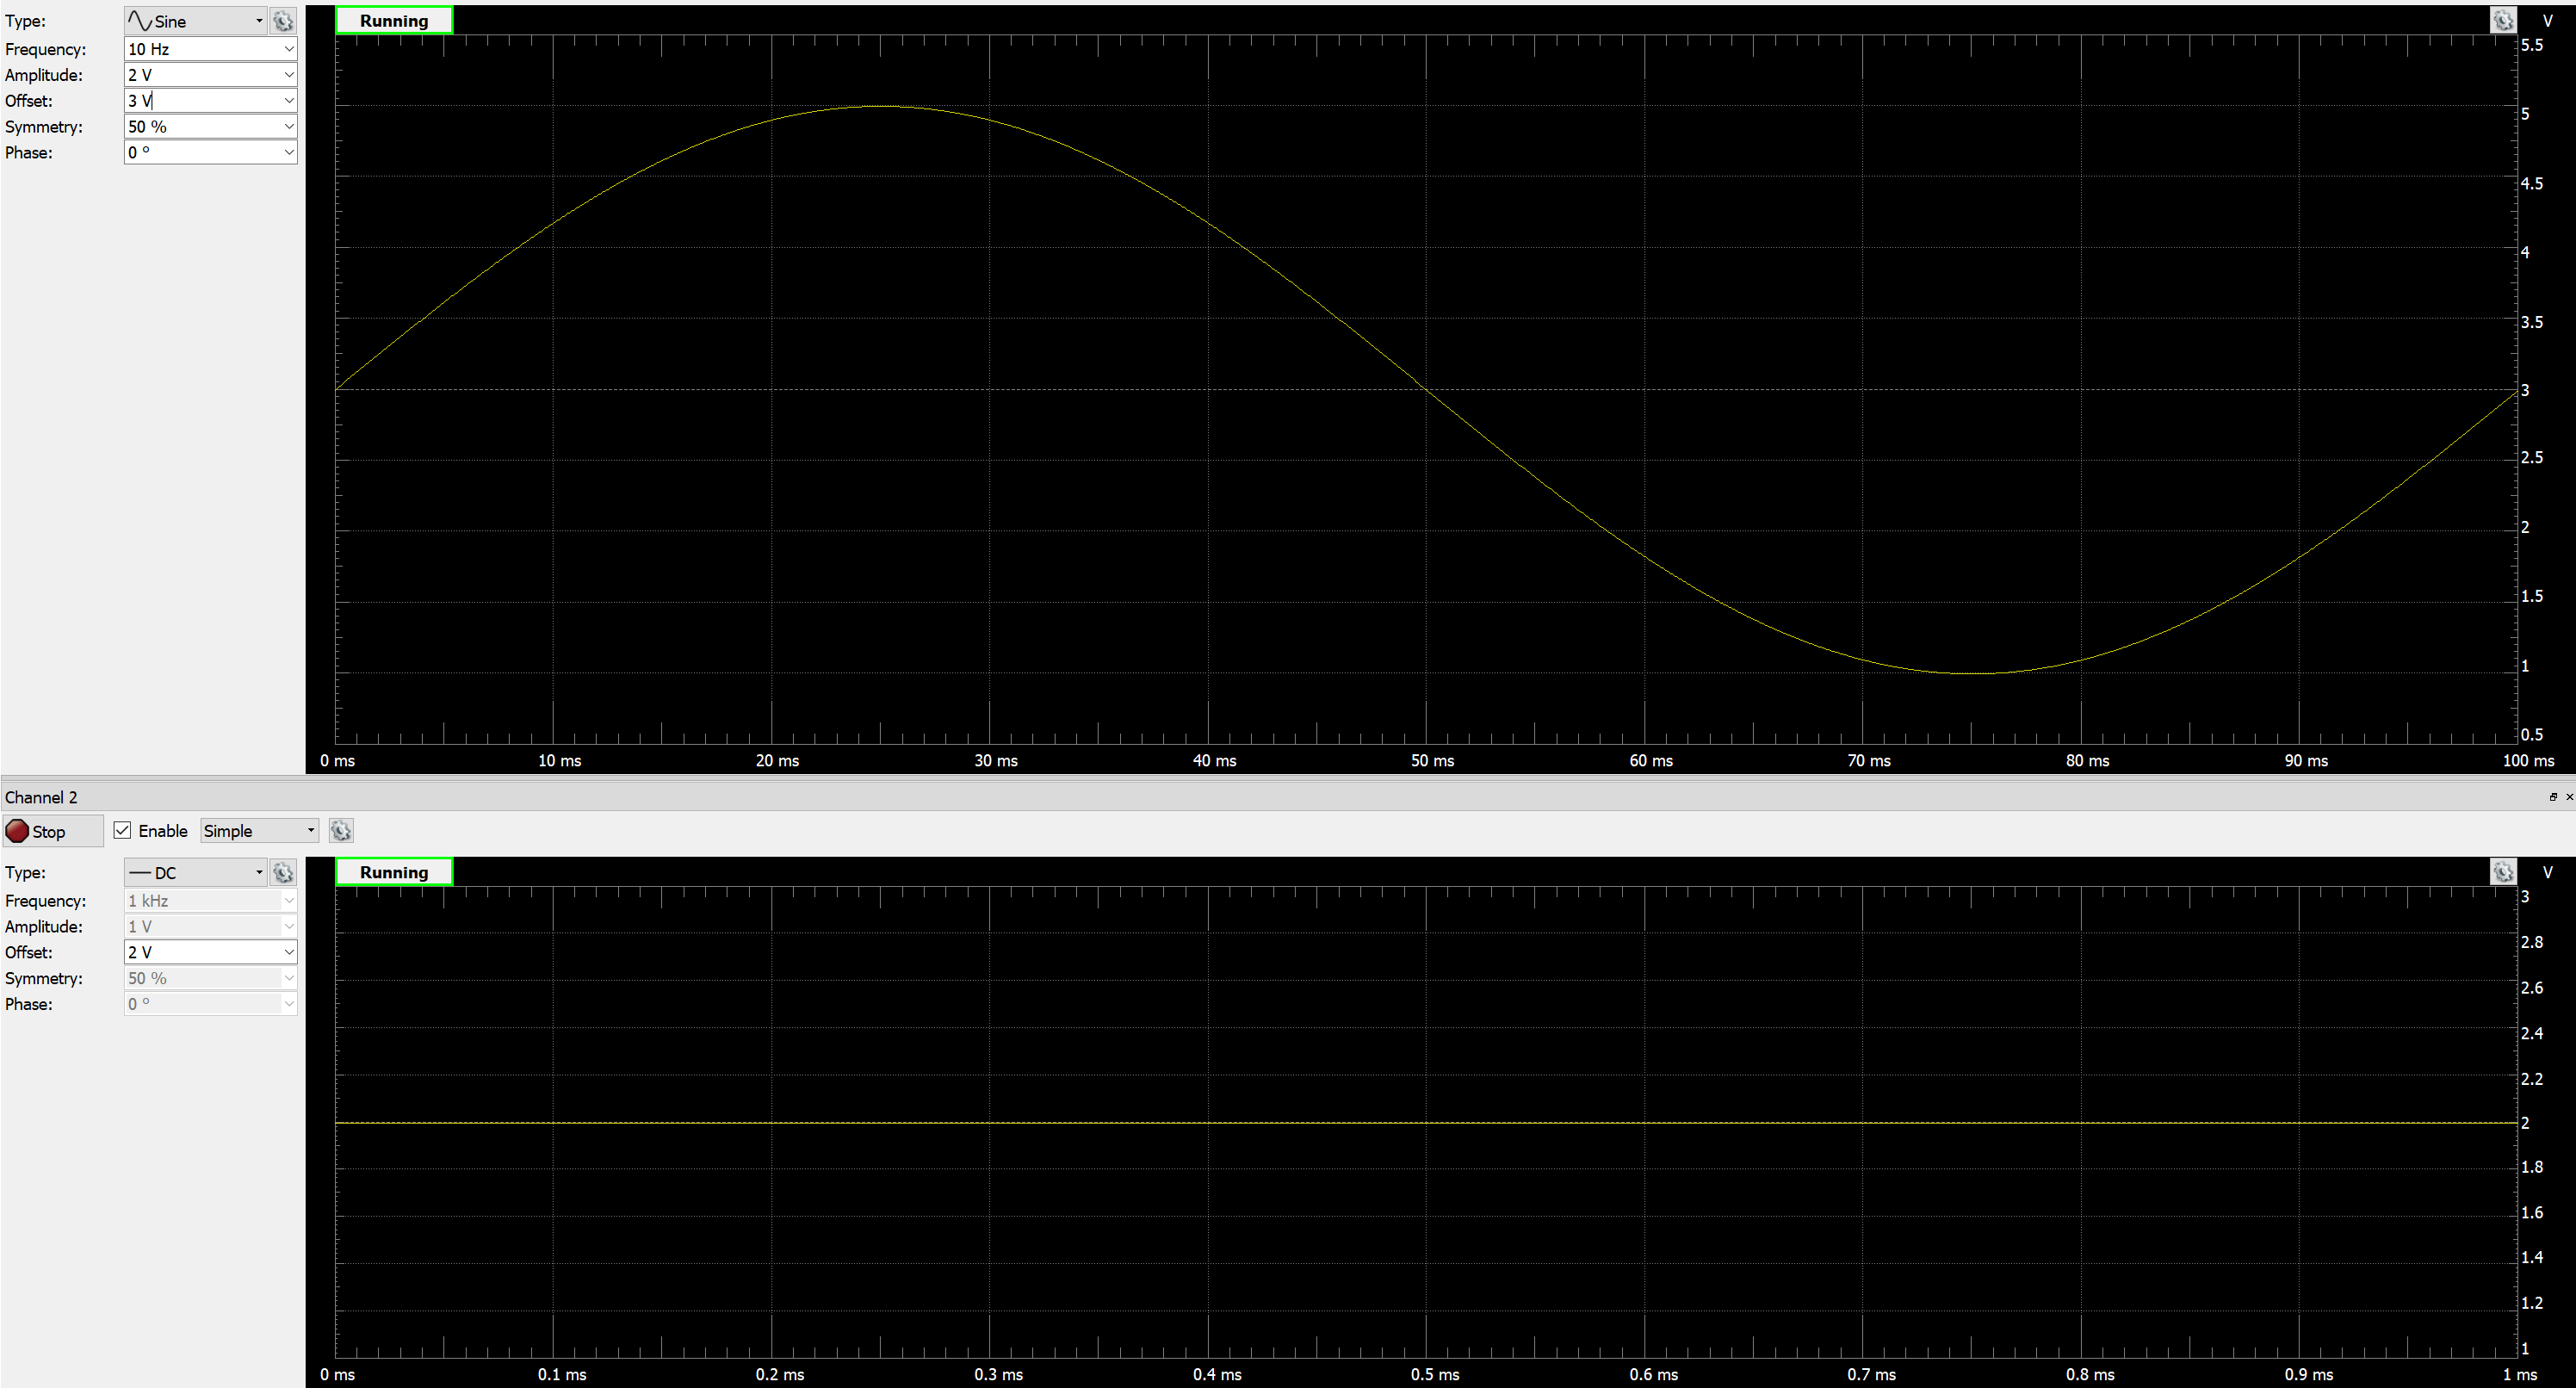
\includegraphics[width=1\linewidth]{Hardwaredesign/Subtractor3}
	\caption{Test af subtractor - offset 3V}
	\label{fig:Subtractor3}
\end{figure}

\begin{figure}[h!]
	\centering
	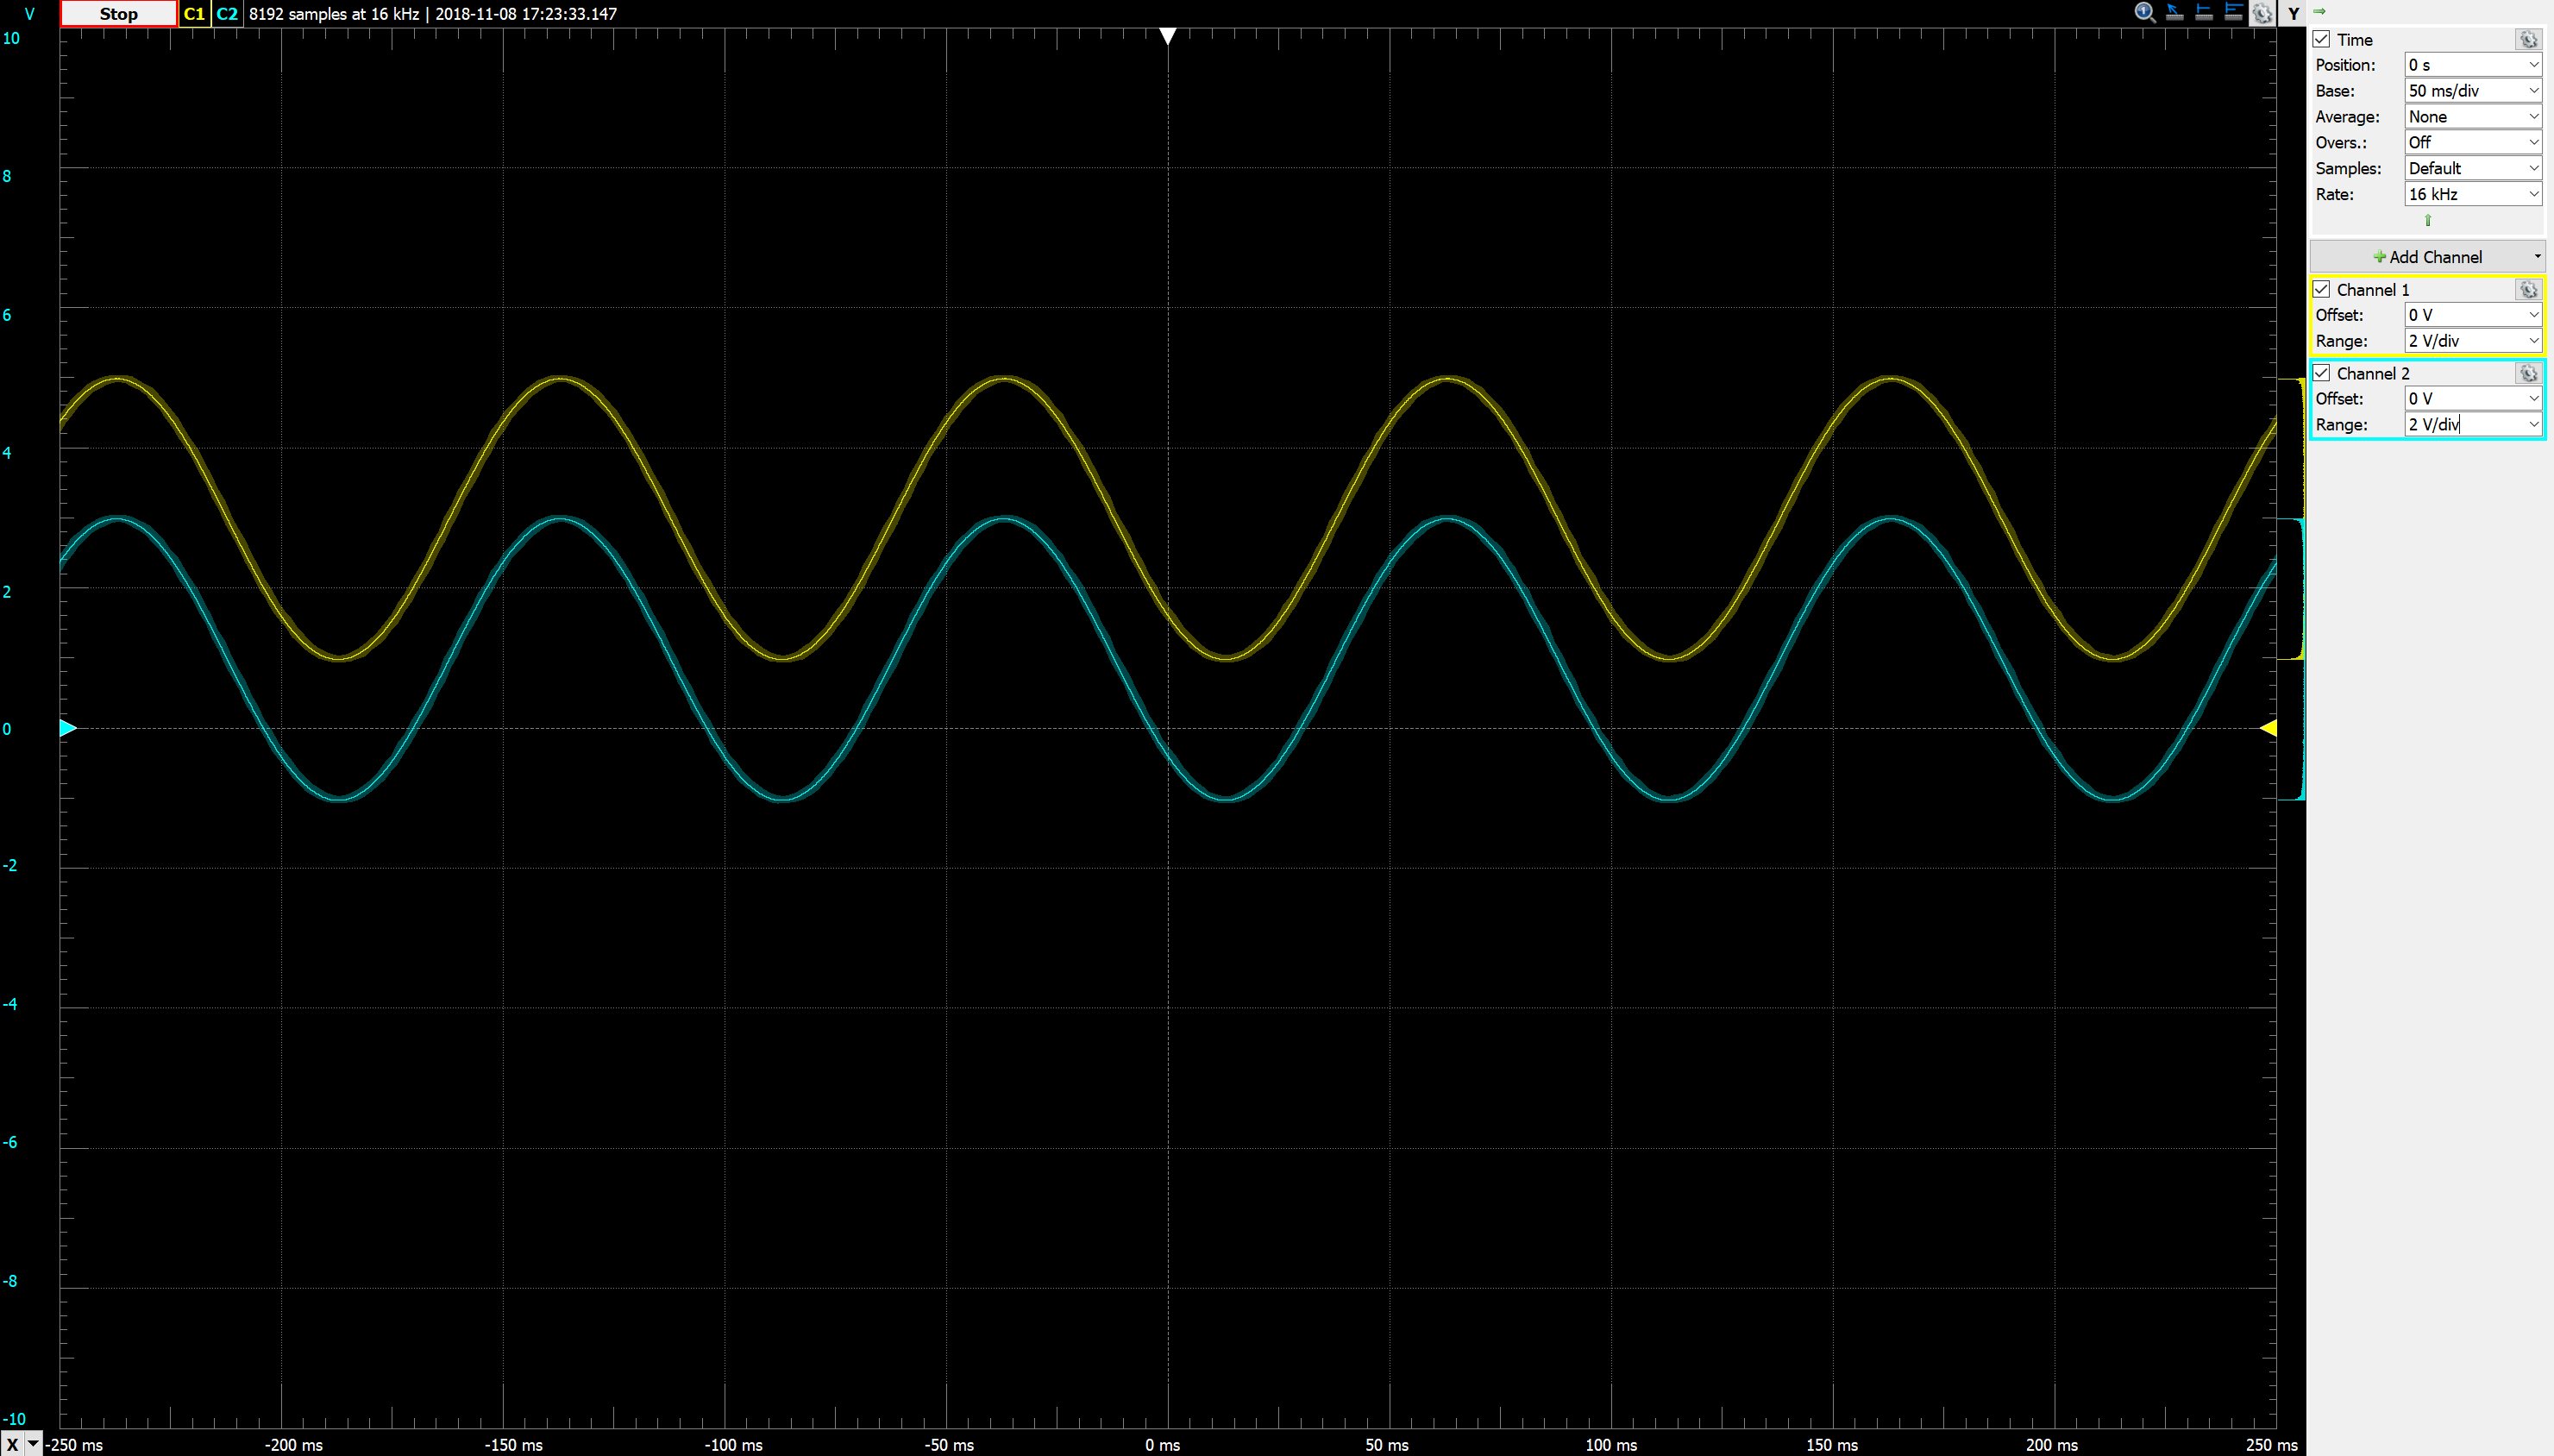
\includegraphics[width=1\linewidth]{Hardwaredesign/Subtractor4}
	\caption{Test af subtractor - offset 3V}
	\label{fig:Subtractor4}
\end{figure}